%----------------------------------------------------------------------------
\chapter{Design and implementation}
\label{chap:designimplementation}
%----------------------------------------------------------------------------

Let's recap the task flow of the task I described in the Introduction: After
configuring the simulator with the designed camera setting I render multiple
traffic scenarios in different maps provided by CARLA while extracting all
necessary information into a log file to later compare the detection log with


\begin{figure}[!ht]
    \centering
    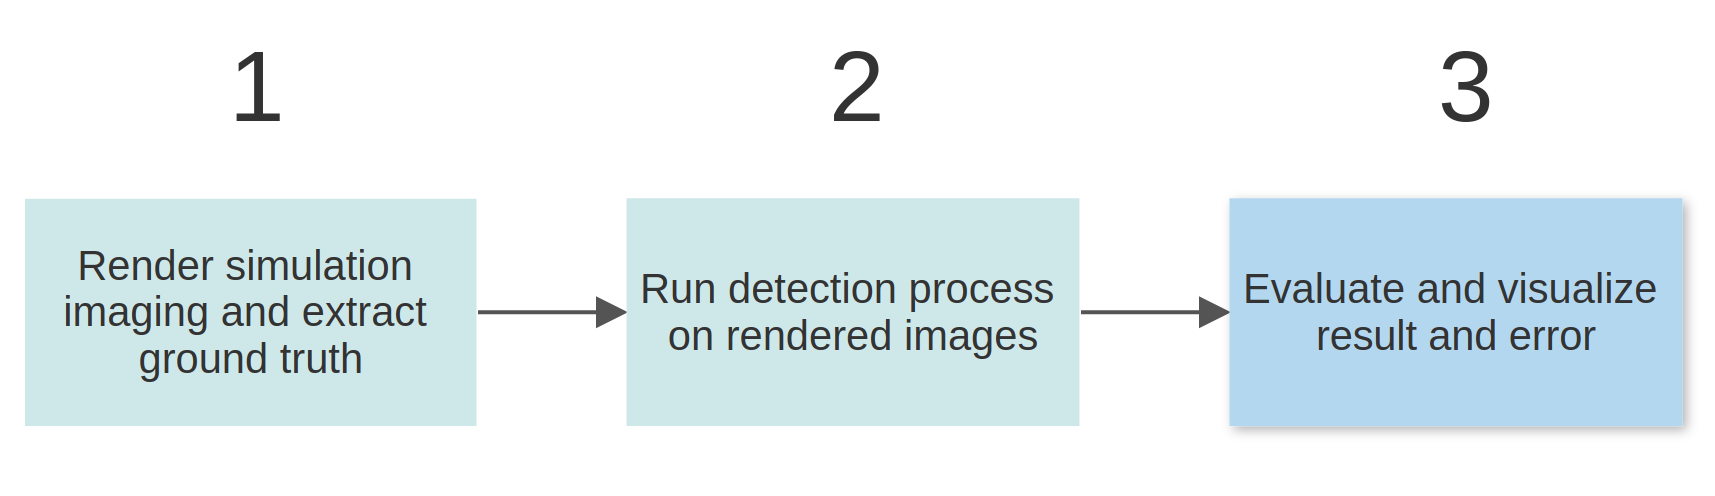
\includegraphics[width=150mm, keepaspectratio]{figures/flowchart.png}
    \caption{Task flow}
    \label{fig:flow2}
\end{figure}


\section{Tools used}

Very soon it became obvious that Linux operating system is the right tool to use
for development. I have been using Ubuntu before this project as well so I was
already familiar with everything. The main IDE I used throughout the project is
Visual Studio Code, which thanks to it's openness and community has a lot of
extensions that helped me develop in fact every part of the thesis: Python,
Nodejs and Javascript for the webvisualizer and finally LaTeX and ofcourse git
support.

I also used Conda which is I think an essential tool when you want to develop ML
and AI projects with Python. Conda makes it easy to create and use separate
Python environments. This is very important because different implementations of
algorithms require different versions of the same packages thus it keeps a clean
separation. The drawback is that consecuently it requires a lot of drive memory.

Upon developing the algorithm and experimenting with it I used Jupyter Notebook
which is a Python runtime on top of the bare one and a web-based IDE at the same
time. With Jupyter Notebook it is very easy to change and re run the code thanks
to it's "kernel" system, which keeps the value of variable and imported packages
between executions.

For the GPU-intensive tasks such as simulation and convnet calculations in the
detector I was provided with a remote Titan X GPU\footnote{ Titan X GPU
    \url{https://www.nvidia.com/en-us/geforce/products/10series/titan-x-pascal/}} by
my university.

\section{Choosing the sensor suite}

Mounting cameras around the vehicle to have an all around vision is an essential
design strategy, as we have seen in the work of other companies in
\autoref{chap:relatedwork}. However we will need to determine depth as well. I
decided to use only cameras in a stereoscopic structure to create 4 stereo sides
around the vehicle. The following image shows the design setting with field of
views visualized in \refstruc{fig:3dmodel3}.

\begin{figure}[!ht]
    \centering
    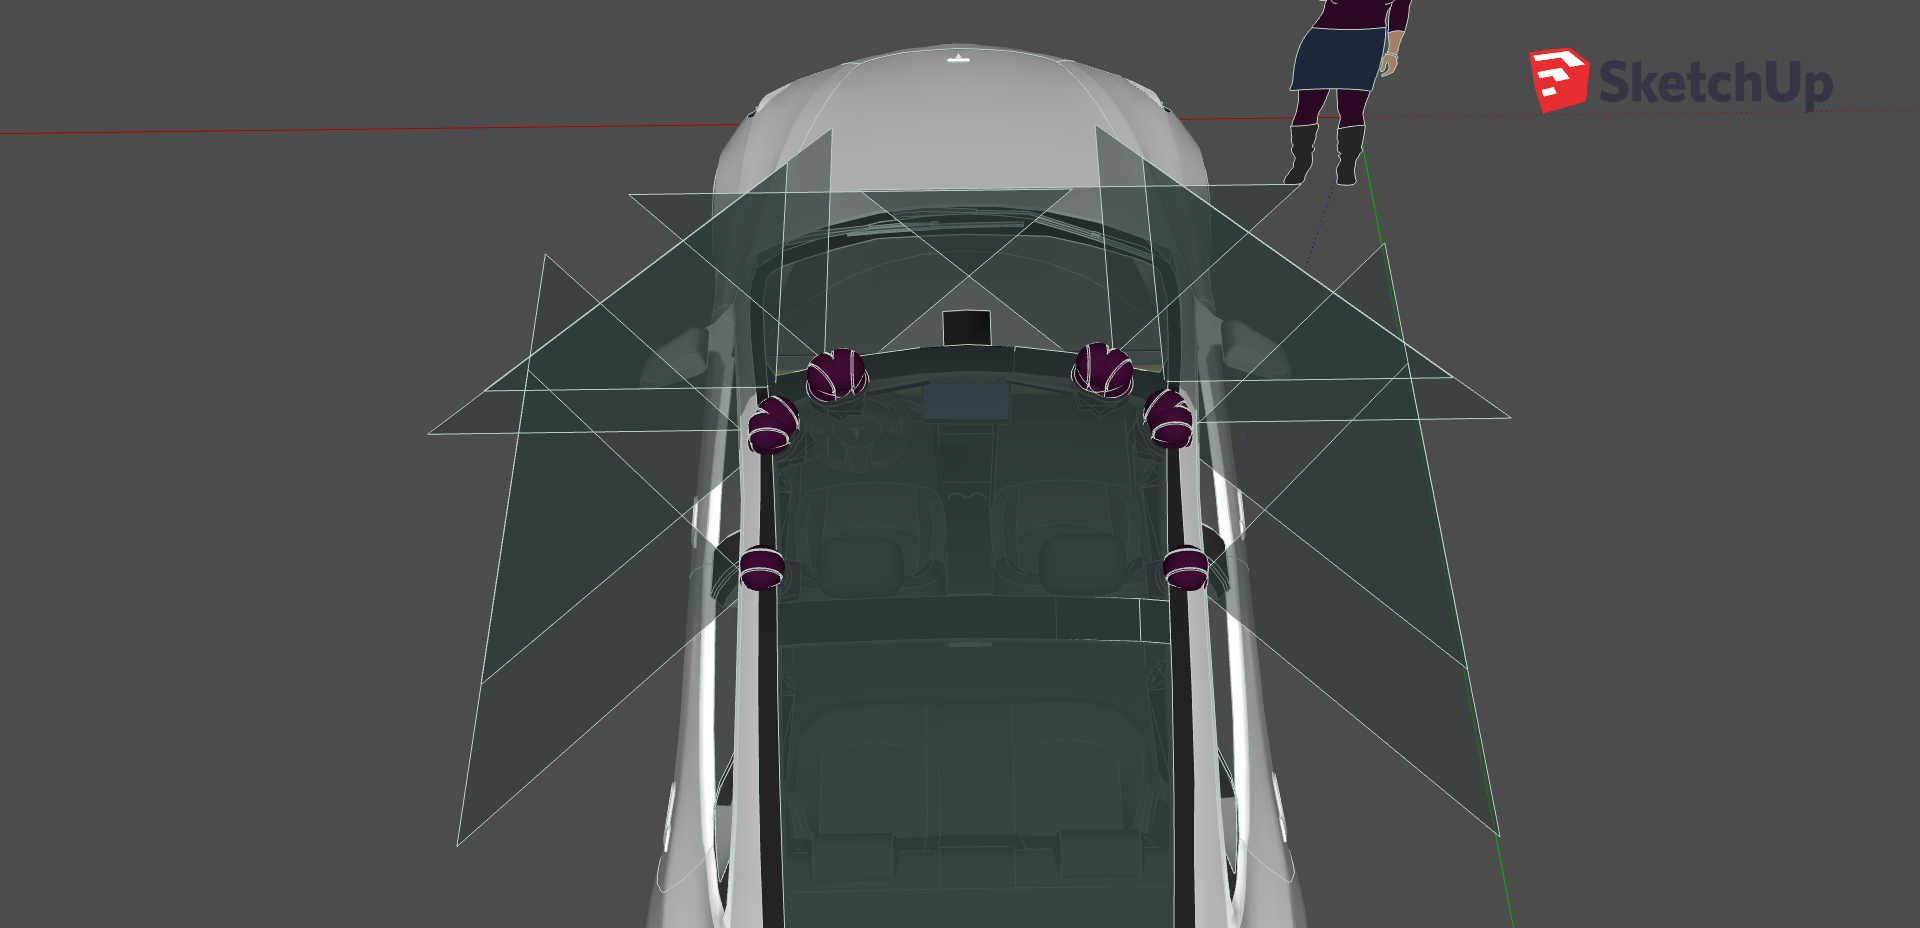
\includegraphics[width=150mm, keepaspectratio]{figures/3dmodel3.png}
    \caption{The stereo camera setting I used on top of the virtual Tesla Model 3}
    \label{fig:3dmodel3}
\end{figure}

In details: 
\begin{itemize}
    \item Front stereo: two cameras looking straight to the front 0.8 meters
          apart
    \item Right corner and left corner stereo cameras: the cameras are on the
          diagonal corners of a 20 cm wide 20cm tall triangle creating two 45\degree
          angled stero vision.
    \item Right and left side stereos are turned 90\degree to the sides and they are apart 0.5 meter.
\end{itemize}
The cameras are 1.5 meters above the ground.

The advantage of puting stereo cameras apart to a relatively large distance is
that it increases the accuracy of the stereo block matching algorithm to a
further distances. The drawback however is that a smaller portion of the right
and left side images are going to intersect hence creating a smaller field of
view. However due to the corner stereo cameras this is not a problem for us.

\section{Configuring the simulation}

Carla simulator can be ran in two time-step settings: variable and synchronous.
In real-world perception it is a complex task by itself to synchronize multiple
cameras with each other so that when the algorithm calculates information based
on data from multiple sensors they all correspond to the same moment in time
with an error boundary. In a simulation however we can have the freedom to
synchronize the simulation timesteps themselves and collect all imaging data
between each timestep. Setting Carla to synchronous timestep ensures that all
images in a certain frame are collected and respond to the same moment. 

I used 30FPS timestep setting so that physics calculations are still realistic
but the performance is not too bad. We also have to account for the size of the
generated images: it was good to half the size of the image datasets from a
60FPS setting. Increasing the traffic participants also degrades the
performance. I usually used 200 vehicles and 100 pedestrians for each map, that
resulted in realistic traffic scenarios. 

I recorded different scenarios of approximately 1 minute, which means 1800
frames on 30FPS. On the Titan X machine it it took 15 minutes to render 1
simulation minute, i.e. it ran the simulation with 2FPS. Note, this is different
from the simulation time-step which we fixed to 30FPS.  Since I collect 10 images
in each frame it results in a dataset of 18000 images.

The camera setting I used is an undistorted camera that takes 1280x720
resolution images, i.e HD 720p images, compressed with JPEG to yield a
reasonable size. This way one image is on average 215 kilobytes instead of 1MB
which is a very good compression rate and this was the limit where I did not see
any difference in detection accuracy.

In a real-world systems images go straight to the GPU and CPU unit and they get
downscaled to the choosen size before feeding into the algorithm. I had to
resort to compression because of the research nature of the project: I reran
and tested the accuracy of the detector many times on the same dataset.

Using an undistorted camera matrix only means that we need to use one less back
transformation matrix in the detection calculations. In real-world the intrinsic
camera matrix is calculated and corrected for cameras that are mounted on cars
and it is part of the calculation.

Besides imaging we have the ground truth log data. During the simulation,
besides rendering images I coded a logger that logs the necessary information of
the state of the simulator for each frame. This information is built up in a
json-like dictionary, and at the end of the simulation it is saved to one file,
that I call the framelist.

\section{Extracted data}

Naming the images in an organized way is important to make it easy to read the
images in a structured way upon detection. Each image starts with the number of
the frame it was taken in. Starting the simulator server Carla increases a
frame counter starting with 1. To know which image corresponds to which camera,
the framenumbers are postfixed with a label. \refstruc{fig:labeling} shows the
postfixes for each image.

\begin{figure}[!ht]
    \centering
    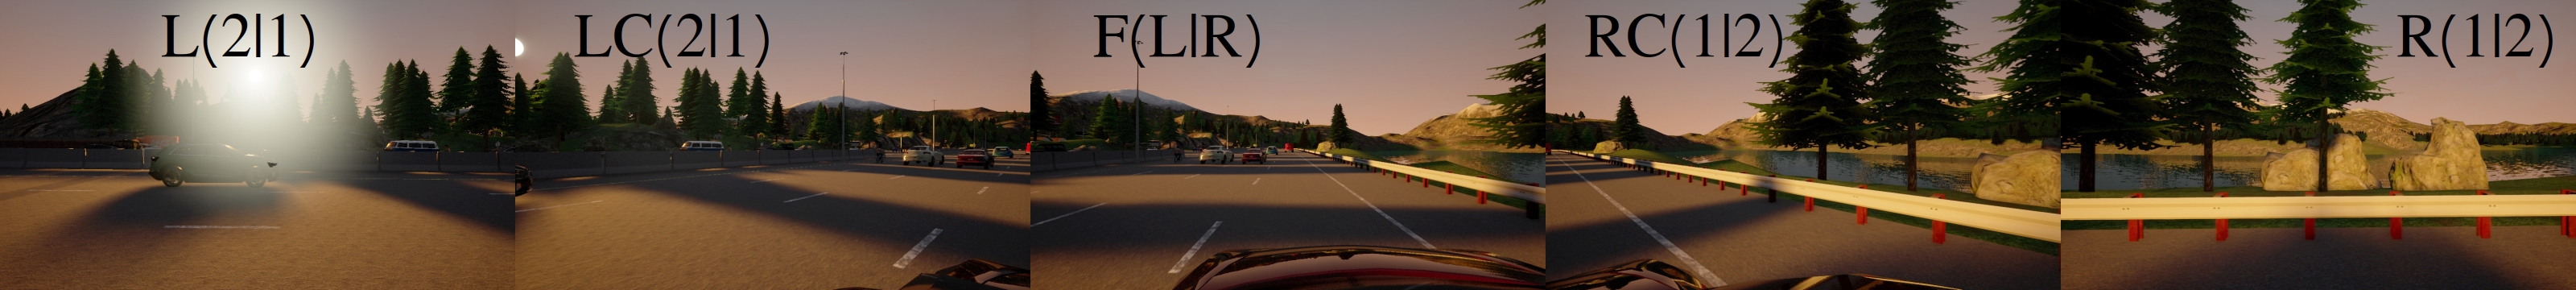
\includegraphics[width=150mm, keepaspectratio]{figures/labeling.jpg}
    \caption{L2/1, R1/2: Right side/Left side first and second cameras, LC(2/1), RC(1/2): Right corner, left corner cameras, FL FR: Front left, front right cameras}
    \label{fig:labeling}
\end{figure}

In each frame I log information about the current state of the simulation. For
the purpouses of the final detector the following information gets logged in each frame:
\begin{itemize}
    \item Frame's number: the value of the frame counter at each frame
    \item For all walker and vehicle actors in a 100 meter radius from the ego car: 
    \begin{itemize}
        \item Id: corresponds to the actor's unique id among other actors.
        \item Relative position: X, Y, Z coordinate of the actor in the CARLA
        coordinate system (see \refstruc{fig:carlacoords})
        \item Distance: Euclidean distance from the ego car 
      \end{itemize}
    \item Waypoints: these are center and left-right points of the lane the egocar is currently in up
    to 30 points forward. These were meant to be the ground-truth data for
    lane-detection
\end{itemize}

This information is then exported into a JSON file with the following format:
\begin{lstlisting}[language=]
frameList: [
    {
        frame: Number,
        actors: [
            {
                type: car|pedestrian,
                id: Number,
                relative_position: {
                    x: Number,
                    y: Number,
                    z: Number,
                }
            },
        ],
    },
]
\end{lstlisting}

For a one-minute simulation the ground-truth json file is approximately 20
megabytes. It isn't optimal to save information like this for longer
simulations. In those cases it is recommended to use a binary format. Carla
provides a way to save binary information of the recording but unfortunately
there were issues with recording that way, so I ended up with this custom log
format. However it ended up being very beneficial, because the webvisualizer
simply loads the json files (detection and ground truth) into two JavaScript
objects.

\section{Detector}


The plan: 
three images of detection montage!!!

\subsection{OpenCV}
Intro to it
\subsection{Detectron2}
- Occulsion
- Detection images!
- Pretrained models
- Comparison
- Object detection and localization
- Instance segmentation
\subsection{Depth estimation}
\subsubsection{Triangulation}
- Triangulation
\subsubsection{Stereo Block Matching Algorithm}
- Stereo Block Matching Algorithm (newer)
\subsubsection{Result}
- 
\subsection{Back projection}
- Camera model and coordinates

- Camera setting
- Inverse transformation explain, Translation: same matrix as camera why
- Yaw pitch roll, euler matrix
- Affine matrix

\subsection{Final pseudo-code}
Final pseudo code
\begin{lstlisting}[language=]
       pseudo code
    \end{lstlisting}

\section{Web visualizer}
In order to measure the accuracy
Web visualizer
-  Framework
-  Usage and results

\section{Additonal scripts}
-Start script
-Montage script

